\documentclass{article}

\usepackage{graphicx}
\usepackage{amsmath}
\usepackage{amsfonts}       % blackboard math symbols
%\usepackage{booktabs}       % professional-quality tables
\usepackage{algorithmic}
\usepackage{algorithm}
\usepackage{nicefrac}
\renewcommand{\algorithmicrequire}{\textbf{Input:}}
\renewcommand{\algorithmicensure}{\textbf{Output:}}

\begin{document}

{\centering \Large An algorithm to find the point with minimum norm in a convex polygon on the centered unit square\\}
~\\
The presented method finds among the points that belong to a convex polygon and the centered unit square in the Euclidean plane the one point with minimum distance to the origin (as Figure \ref{fig:minNorm} illustrates).
Being very similar to previous work \cite{van2011reciprocal}, the method sligthly varies the approach of incremental linear programming \cite{seidel1991small}, \cite{van2008computational}.

Algorithm \ref{alg:incrementation} receives the convex polygon as a set of halfplanes $ \left\{\tilde H_j\right\}_{j=1}^{m}$ whose intersection defines the polygon. It augments these constraints by the halfplanes $ \left\{H_k^s\right\}_{k=1}^{4}$ whose intersection defines the centered unit square.
To find the solution, it requires to know the solution of the same problem with one constraining halfplane less and which is the respective halfplane. The algorithm allows to incrementally build the final solution for any convex polygon, by solving first the problem without any constraints, then adding one more halfplane and solving again, and so on, until it has processed all the halfplanes. Algorithm \ref{alg:incrementalMin} implements this approach.
\begin{figure}[b!]
	\centering
	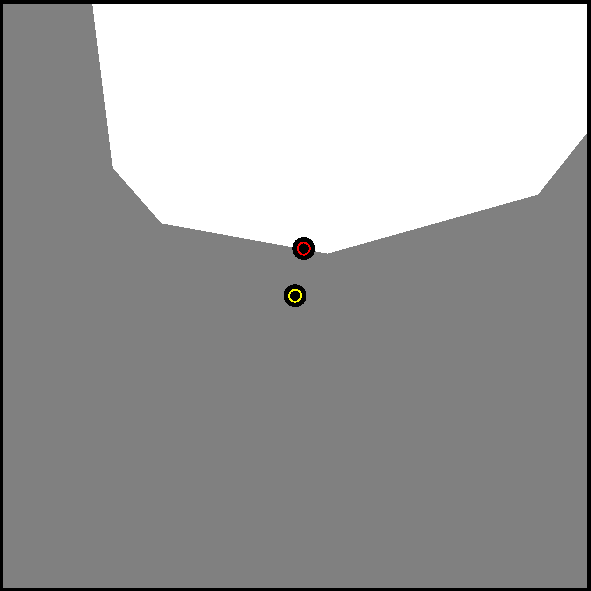
\includegraphics[scale=0.7]{../distance_minimization_unit_square.pdf}
	\caption{The centered unit square (grey), with side length equal to one, and a superposed convex polygon (white). The points indicate the coordinate origin (yellow-black) and its closest point (red-black) belonging to the convex polygon and the unit square.}\label{fig:minNorm}
\end{figure}

\begin{algorithm}[h!]
	\caption{Incremental Distance Minimization}
	\label{alg:incrementalMin}
	\begin{algorithmic}
		\REQUIRE 	halfplanes $ \left\{ H_i\right\}_{i=1}^{n}$
		\ENSURE 	point $ p^* $ closest to $ (0,0) $ while belonging to $ \bigcap\limits_{k=1}^{4} H_k^s \bigcap\limits_{i=1}^{n} H_i$
		\STATE $ p^* \leftarrow (0,0) $
		\FOR { $ i \leftarrow  1, ..., n $ }
		\STATE $ p^* \leftarrow \text{distanceMinimizationIncrementation}\left(H_i, p^*, \left\{ H_j\right\}_{j=1}^{i-1}\right) $
		\ENDFOR
		\RETURN $ p^* $
	\end{algorithmic}
\end{algorithm}

The design of Algorithm \ref{alg:incrementation} allows to avoid numerical problems implied by intersections between (close-to) parallel lines using a simple trick. Namely, one can introduce a small distance tolerance $ \delta $ to bias every query whether a halfplane contains a point (i.e. every halfplane is enlarged by $\delta$ only while performing this check). This allows then to introduce a lower threshold $ \alpha $ for the angle between two boundary lines which Algorithm \ref{alg:incrementation} attempts to intersect. The algorithm can directly report that the problem is infeasible, whenever an attempt occurs for an angle below $ \alpha $, which needs to be chosen as $ \alpha = \sin^{-1}\left( \nicefrac{\delta}{\sqrt{2}} \right) $. This value for $ \alpha $ guarantees that angles below would make the intersection point lie outside the feasible unit square. Thus, the algorithm never has to perform line intersections for very small angles. One can implement Algorithm \ref{alg:incrementation} in a robust way by incorporating this feature, which the pseudo-code omits for the sake of simplicity.

\begin{algorithm}
\caption{Distance Minimization Incrementation}
\label{alg:incrementation}
\begin{algorithmic}
\REQUIRE 	halfplane $ H $, prior solution $\tilde p^* $, prior halfplanes $ \left\{\tilde H_j\right\}_{j=1}^{m}$
\ENSURE 	point $ p^* $ closest to $ (0,0) $ while belonging to $ \bigcap\limits_{k=1}^{4} H_k^s \bigcap\limits_{j=1}^{m} \tilde H_j \cap H $
\STATE $ p^* \leftarrow \tilde p^* $ //\textit{initialize the solution as the prior solution}
\IF	{$ p^* \notin H $}
	\STATE $ p^* \leftarrow \text{projectOriginOrthogonallyOnHalfplaneBoundary}(H) $
	\STATE $ p_1 \leftarrow \text{pointShiftedAlongBoundaryBy} (p^*, H, +\sqrt{2}) $
	\STATE $ p_2 \leftarrow \text{pointShiftedAlongBoundaryBy} (p^*, H, -\sqrt{2}) $
	\FOR { $ k \leftarrow  1, ..., 4 $ }
		\IF		{$ (p_1 \notin H_k^s) \,\&\, (p_2 \in H_k^s) $}
			\STATE $  p_1 \leftarrow \text{intersectHalfplaneBoundaries}(H_k^s, H) $ //\textit{update segment $ [p_1, p_2] $}
		\ELSIF		{$ (p_1 \in H_k^s) \,\&\, (p_2 \notin H_k^s) $}
			\STATE $ p_2 \leftarrow \text{intersectHalfplaneBoundaries}(H_k^s, H) $ //\textit{update segment $ [p_1, p_2] $}
		\ELSIF		{$ (p_1 \notin H_k^s) \,\&\, (p_2 \notin H_k^s) $}
			\STATE \textbf{except} ``infeasible'' //\textit{terminate; $ p_1 $, $ p_2 $ serve only to determine this}
		\ENDIF
		\IF	{$ p^* \notin H_k^s $}
			\STATE $ p^* \leftarrow \text{intersectHalfplaneBoundaries}(H_k^s, H) $ //\textit{update the solution}
		\ENDIF
	\ENDFOR
	\FOR { $ j \leftarrow  1, ..., m $ }
		\IF		{$ (p_1 \notin \tilde H_j) \,\&\, (p_2 \in \tilde H_j) $}
			\STATE $  p_1 \leftarrow \text{intersectHalfplaneBoundaries}(\tilde H_j, H) $ //\textit{update segment $ [p_1, p_2] $}
		\ELSIF		{$ (p_1 \in \tilde H_j) \,\&\, (p_2 \notin \tilde H_j) $}
			\STATE $ p_2 \leftarrow \text{intersectHalfplaneBoundaries}(\tilde H_j, H) $ //\textit{update segment $ [p_1, p_2] $}
		\ELSIF		{$ (p_1 \notin \tilde H_j) \,\&\, (p_2 \notin \tilde H_j) $}
			\STATE \textbf{except} ``infeasible'' //\textit{terminate; $ p_1 $, $ p_2 $ serve only to determine this}
			%\RETURN ``infeasible'' //\textit{$ p_1 $ and $ p_2 $ serve only to determine this}
		\ENDIF
		\IF	{$ p^* \notin \tilde H_j $}
			\STATE $ p^* \leftarrow \text{intersectHalfplaneBoundaries}(\tilde H_j, H) $ //\textit{update the solution}
		\ENDIF
	\ENDFOR
\ENDIF
\RETURN $ p^* $
\end{algorithmic}
\end{algorithm}

\bibliographystyle{ieeetr}
\bibliography{references}

\end{document}